\begin{center}
	\pagecolor{deepred}
	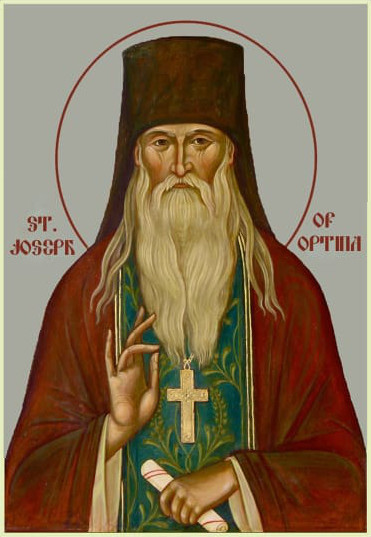
\includegraphics[width=\textwidth]{Images/StJosephOfOptina.jpg}
    
    \vspace*{\fill}

	\color{white}\LARGE \textbf{THE ELDER JOSEPH OF OPTINA}
\end{center}
\clearpage
\pagecolor{white}

\begin{adjustwidth}{.5cm}{.5cm}\itshape
	
	Editorial Note: 

    The following is an amateur reproduction of "The Elder Joseph of Optina", created out of a love for St. Joseph
    in the hope that others who would like to learn about his life can do so more easily than I was able to as this book has been 
    out of print for many years. When I finally found a copy I photographed each page and ran the photos
    through OCR software to extract the text, manually fixing the copious associated errors.

	While the text is as true to the original as possible, the page numbers do not match due to typesetting
	differences. I also left out many of the decorative images, 
	but included the original photos of people and places discussed. Original copyright info below.
	
	Please forgive any shortcomings, flaws, and mistakes. May God accept this small effort, 
	provide the correction and perfection it needs as he sees fit, and forgive my many offenses.\\
    \\
    St. Joseph, pray for us.\hspace*{\fill}-- Irenei\hspace*{1cm}
	
\end{adjustwidth}
\vspace*{\fill}
\begin{center}
	
	ISBN: 0-913206-53-0\\
	Library of Congress Catalog Card Number: 82-81456\\
	Holy Transfiguration Monastery, Brookline MA 02146\\
	Translation \textcopyright 1984 by the Holy Transfiguration Monastery\\
	All rights reserved\\
	Printed in the United States of America
\end{center}
\clearpage
